\begin{tikzpicture}
	\node[inner sep=0pt, anchor=north west] (raw) at ( 0.0, 0)
		{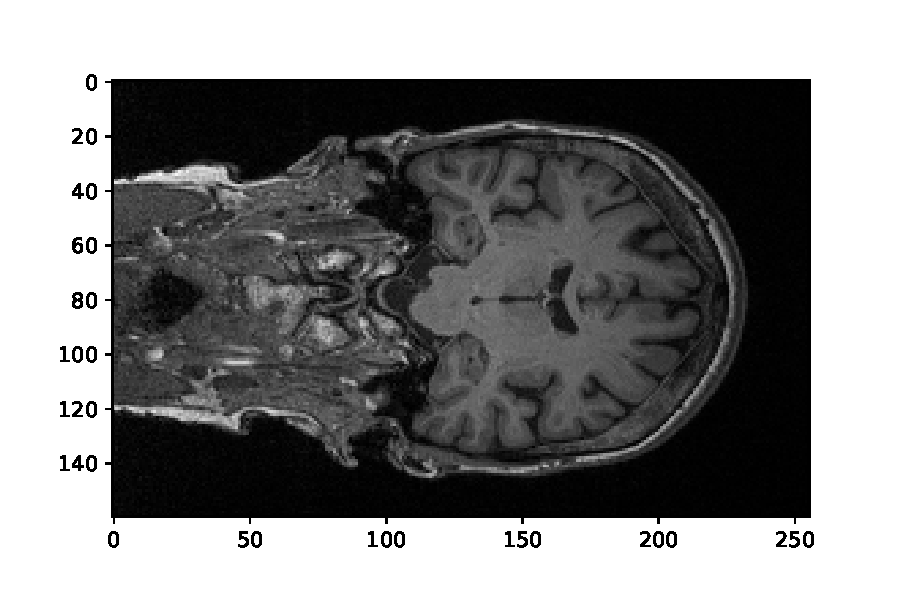
\includegraphics[height=.4\textwidth, trim={18 0 0 0}, clip]{images/preproc/raw.pdf}};
	\node[inner sep=0pt, anchor=north east] (fov) at (16.0, 0)
		{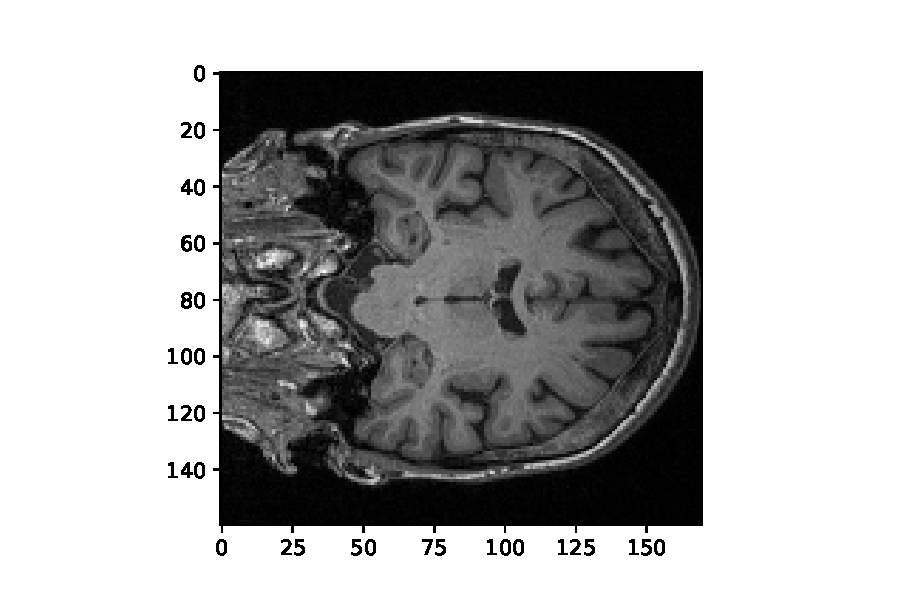
\includegraphics[height=.4\textwidth, trim={60 0 68 0}, clip]{images/preproc/fov.pdf}};
	
	\node[inner sep=0pt, anchor=north east] (fli) at (16.0, -5.75)
		{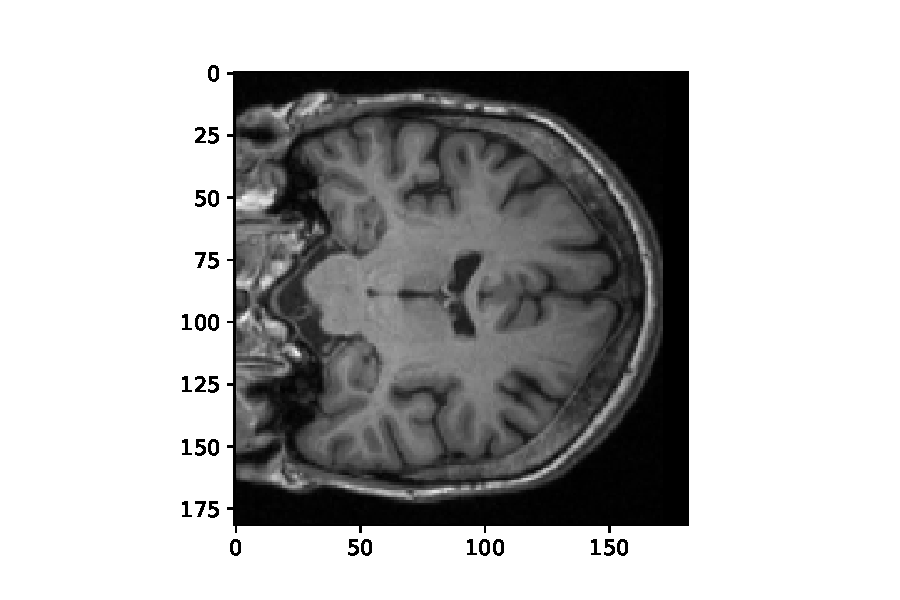
\includegraphics[height=.4\textwidth, trim={75 0 75 0}, clip]{images/preproc/fli.pdf}};
	\node[inner sep=0pt, anchor=north west] (msk) at ( 5.5, -5.75)
		{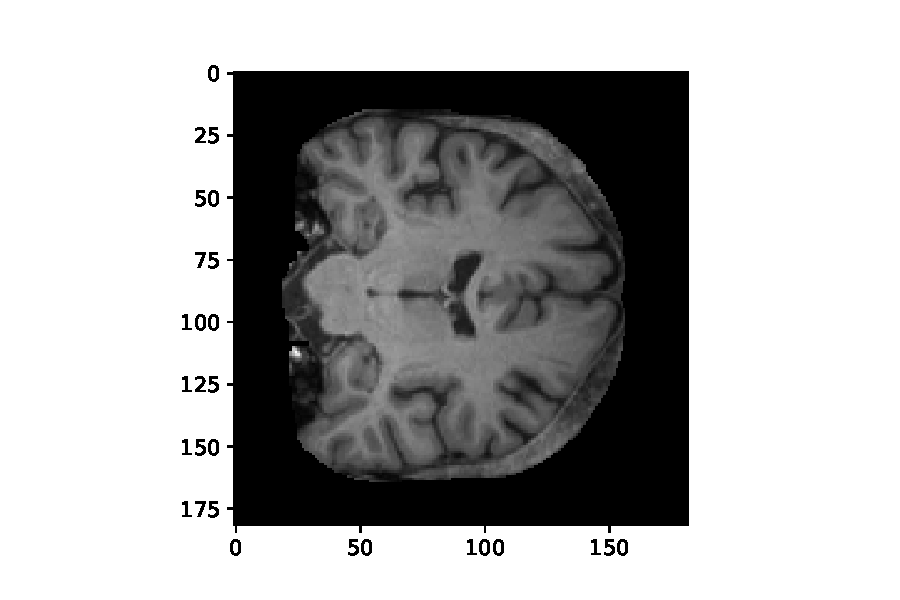
\includegraphics[height=.4\textwidth, trim={75 0 80 0}, clip]{images/preproc/msk.pdf}};
	\node[inner sep=0pt, anchor=north west] (bet) at ( 0.0, -5.75)
		{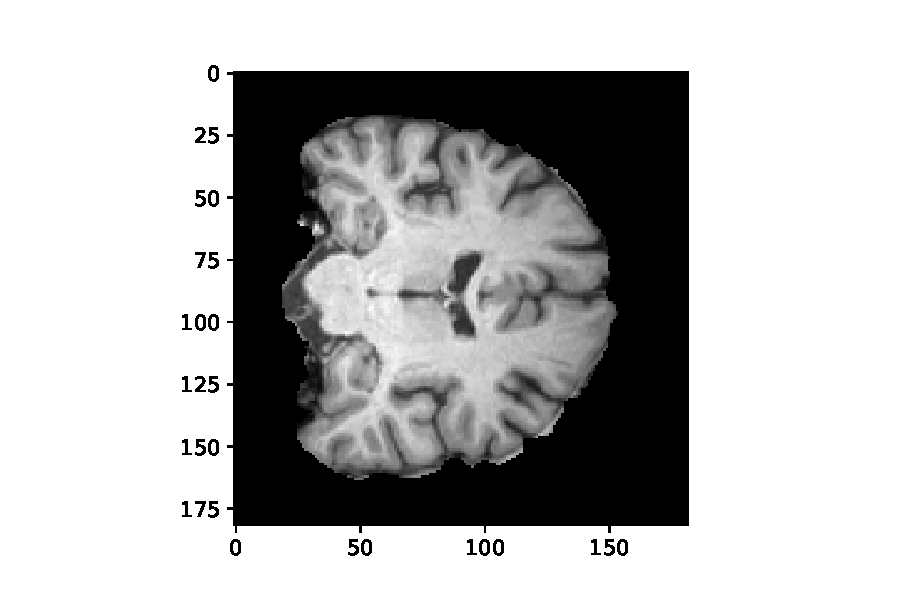
\includegraphics[height=.4\textwidth, trim={75 0 75 0}, clip]{images/preproc/bet.pdf}};

	\node[inner sep=0pt, anchor=north east] (pv1) at (16.0, -12)
		{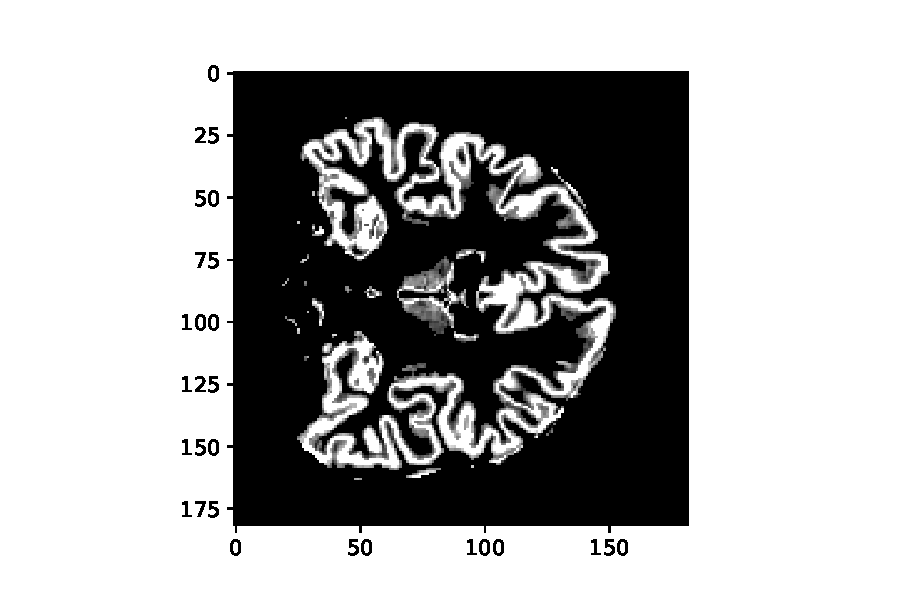
\includegraphics[height=.4\textwidth, trim={75 -10 75 10}, clip]{images/preproc/pve_1.pdf}};
	\node[inner sep=0pt, anchor=north west] (pv2) at ( 5.5, -12)
		{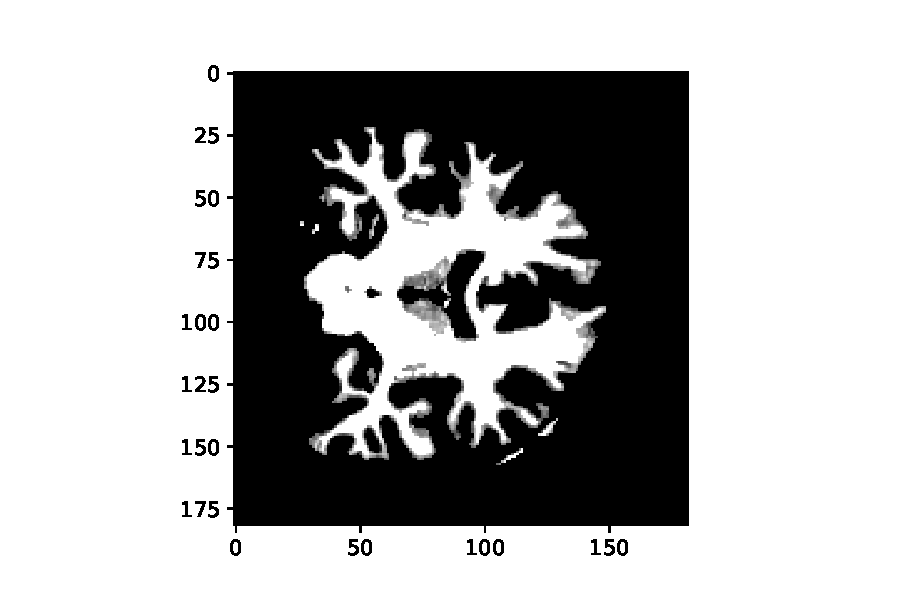
\includegraphics[height=.4\textwidth, trim={75 -10 75 10}, clip]{images/preproc/pve_2.pdf}};
	\node[inner sep=0pt, anchor=north west] (res) at ( 0.0, -12)
		{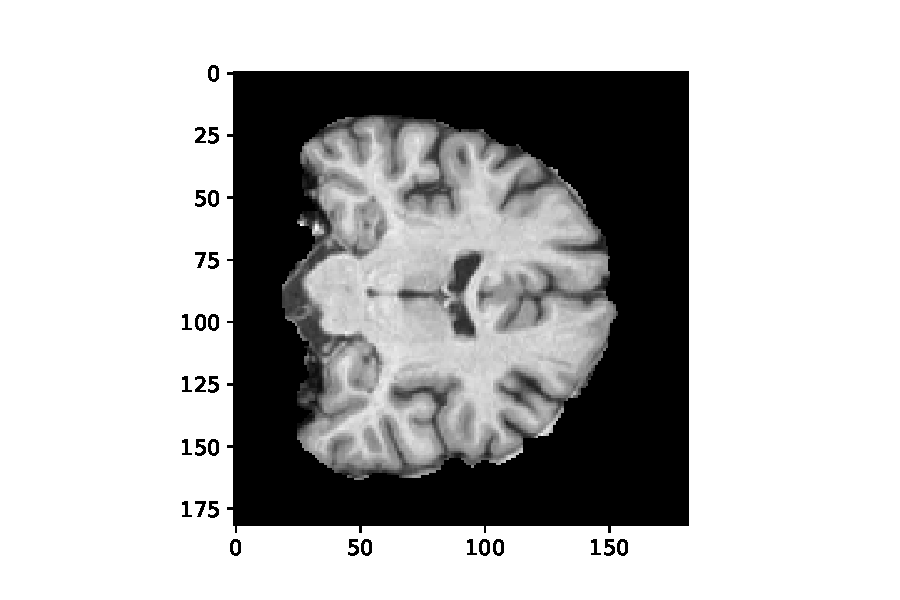
\includegraphics[height=.4\textwidth, trim={75 -10 75 10}, clip]{images/preproc/res.pdf}};
	
	\node[inner sep=0pt, anchor=north]      (sub) at (10.85, -17.75)
		{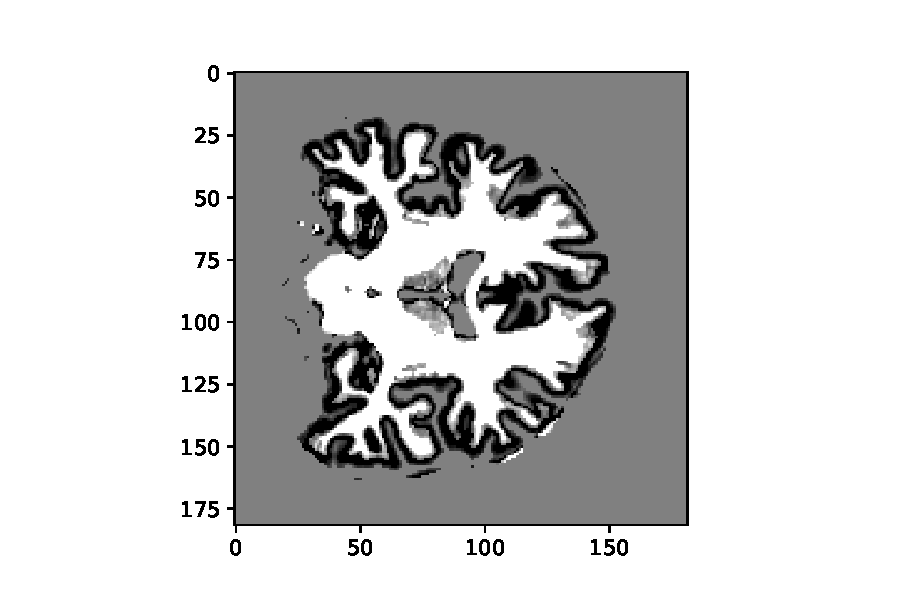
\includegraphics[height=.4\textwidth, trim={75 0 75 10}, clip]{images/preproc/sub.pdf}};

	\draw[->, very thick] (raw) -- node[below=5pt]{\texttt{robustfov}} (fov);
	\draw[->, very thick] (fov) -- node[right=10pt]{\texttt{flirt}} (fli);
	\draw[->, very thick] (fli) -- node[above=10pt, right=0pt, rotate=90]{\texttt{mask}} (msk);
	\draw[->, very thick] (msk) -- node[above=10pt, right=0pt, rotate=90]{\texttt{bet}}(bet);
	\draw[->, very thick] (bet.south) -- (pv1.north);
	\draw[->, very thick] (bet.south) -- (pv2.north);
	\draw[->, very thick] (bet.south) -- node[left=10pt]{\texttt{fast}} (res.north);
	\draw[->, very thick] (pv1) -- node[left=10pt]{\texttt{subtract}} (sub);
	\draw[->, very thick] (pv2) -- (sub);


\end{tikzpicture}
